\documentclass[11pt]{article}
\usepackage{preamble}
\titleformat*{\section}{\Large\bfseries}
\usepackage{mathtools}
\usepackage{listings, courier}
\lstset{basicstyle=\small\ttfamily,breaklines=true}
\lstset{
      numbers=left,
      stepnumber=1,    
      firstnumber=1,
      numberfirstline=true,
      xleftmargin=6em,
      framexleftmargin=3.5em,
      framextopmargin=6pt,
      framexbottommargin=6pt, 
      frame=tb, framerule=0pt,  
      numberstyle=\small\color{gray},
      numbersep=20pt,
      backgroundcolor=\color{gray!10},
}
\DeclarePairedDelimiter\ceil{\lceil}{\rceil}
\DeclarePairedDelimiter\floor{\lfloor}{\rfloor}
\def\columnseprulecolor{\color{blue}}

\title{CISC 3220 Homework Chapter 16}
\author{Rachel Friedman}
\date{May 10, 2020}

\begin{document}
\maketitle
\section*{Exercises 16.3}\nointerlineskip
\noindent \rule{\linewidth}{0.01pt}\\
\subsubsection*{Question 16.3-3}\nointerlineskip
What is an optimal Huffman code for the following set of frequencies, based on the first 8 Fibonacci numbers?\\
\indent \indent \indent a:1 b:1 c:2 d:3 e:5 f:8 g:13 h:21\\
Generalize your answer to find the optimal code when the frequencies are the first $n$ Fibonacci numbers.\\
\begin{center}
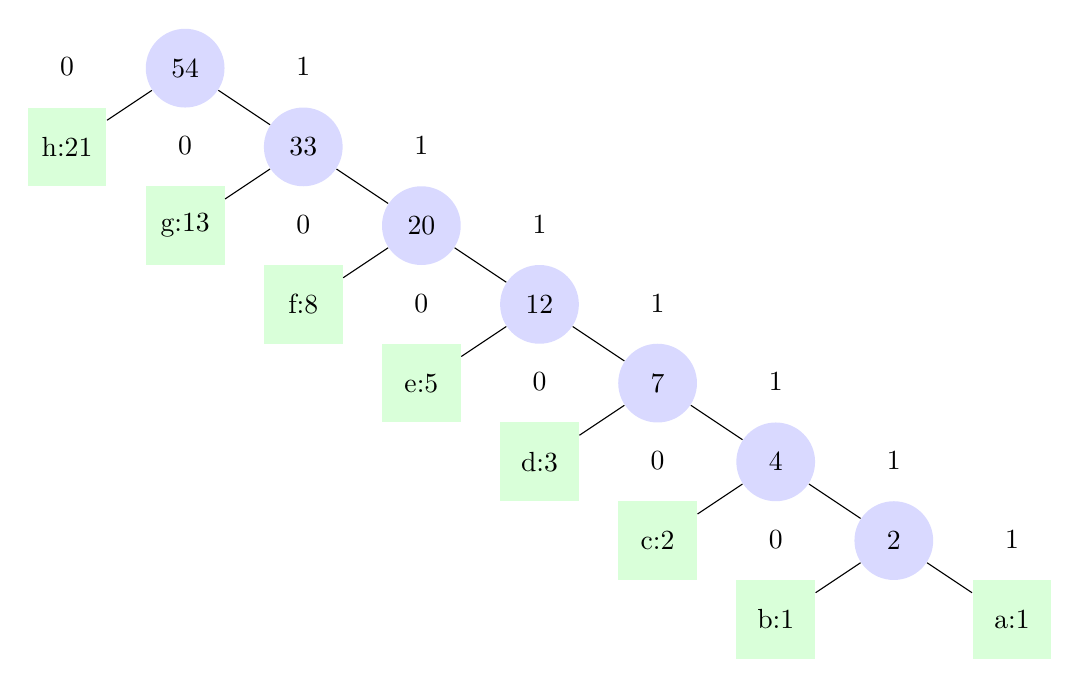
\begin{tikzpicture}
  [level distance = 10mm, node distance=0.1,
   every node/.style={fill=blue!15!white,circle, inner sep=1pt, minimum size=10mm},
   level 1/.style={sibling distance = 30mm},
   level 2/.style={sibling distance = 30mm},
   level 3/.style={sibling distance = 30mm},
   level 4/.style={sibling distance = 30mm}]

  \node {54}
     child {node[fill=green!15!white,rectangle,label=0]{h:21}}
     child {node [label=1] {33}
        child {node[fill=green!15!white,rectangle,label=0]{g:13}}
        child {node [label=1] {20}
            child {node[fill=green!15!white,rectangle,label=0]{f:8}}
            child {node [label=1] {12}
                child {node[fill=green!15!white,rectangle,label=0]{e:5}}
                child{node [label=1] {7}
                    child {node[fill=green!15!white,rectangle,label=0]{d:3}}
                    child {node [label=1] {4}
                        child {node[fill=green!15!white,rectangle,label=0]{c:2}}
                        child {node [label=1] {2}
                            child {node[fill=green!15!white,rectangle,label=0]{b:1}}
                            child { node[fill=green!15!white,rectangle,label=1]{a:1} 
                }}}}}}
     };
\end{tikzpicture}
\end{center}

\begin{multicols}{2}
\noindent a = 1111111\\
b = 1111110\\
c = 111110\\
d = 11110\\
e = 1110\\
f = 110\\
g = 10\\
h = 0\\

This generalizes to the most frequent Fibonacci number having a code of 1 repeated $n-1$ times, and the $n^{th}$ most frequent Fibonacci number having a code of 1 repeated $n-1$ times with the addition of a zero at the end. For instance, in the 8 Fibonacci numbers in this example, since $b$ is the $7^{th}$ most frequent number, its code is six ones and one zero.\\

\end{multicols}
\end{document}